\section{Results}
\label{sec:results}
In this section we briefly survey experimental results appearing in
\cite{Ozkan2014MainEasal,Ozkan2014MC,Wu2014Virus}, that illustrate some of EASAL's
capabilities. The main applications of EASAL are in
estimating free-energy, binding affinity, crucial interactions for assembly,
and kinetics for supramolecular self-assembly starting from rigid molecular
motifs e.g., helices, peptides, ligands etc.

\subsection{Atlasing and Paths} 
\label{sec:atlasandpath}
\begin{table}[h]
\resizebox{\columnwidth}{!}{%
\begin{tabular}{cC{4cm}cccc}\hline
		$n$ & Step size(as a fraction of the smallest radius) & Number of Regions & Number of samples & Good Samples & Time(in minutes)\\\hline\hline
	6 & 0.25  &26k &1.9 million & 1.3 million & 82\\\hline
	6 & 0.375 &23k & 617k & 379k & 23\\\hline
	6 & 0.5 & 19k& 289k & 172k & 11\\\hline
	20& 0.25  & 184k & 5.8 million& 716k & 335\\\hline
	$20^*$  & 0.25  & 206 & 63k & 22k & 2\\\hline
	$20^\dag$ & 0.25  & 3107 & 74k & 33k & 7\\\hline
\end{tabular}
\newline
}

\caption{Time on a standard laptop (see text) to stratify the configuration
space of pairwise constrained point-sets with the tolerance set to $(1.0-0.75)
\times$  sum of radii. The input point-set with $n=6$ is \exref{\toyhelix} and
the $n=20$ input is \exref{\bighelix}. Note that in $20^*$, only one 
5D and its children 4D regions are sampled and in $20^\dag$, only one 5D and its 
descendant 4D and 3D region are sampled.} 
\label{table:stratification}
\end{table}

In this section, we survey numerical results
from experiments in \cite{Ozkan2014MainEasal}, illustrating the performance of
EASAL in generating an atlas and computing paths for the configuration space of
two ($k=2$) input point-sets. The experiments were run on a machine with 
Intel(R) Core(TM) i7-7700 @ 3.60GHz CPU with 16GB of RAM. These results can be
reproduced by the reader using the accompanying EASAL software implementation
(see Section 2.4 of the User Guide for instructions).


The time required for generating the atlas is measured for a given accuracy of
coverage, measured in terms of the step size, and a given tolerance, which is
the width of the interval in \ctwo. Two different input point-sets 
(\exref{\toyhelix} and \exref{\bighelix}) are used as input. The results for 
the $n=6$ input
(\exref{\toyhelix}) show the time and number of
samples for generating the atlas of all possible combinations of active
constraint regions with one active constraint (5D atlas root nodes). The
results for $n=20$ input (\exref{\bighelix}) show the time and number of samples 
required to
generate the atlas for a typical randomly chosen 5D active constraint region and
all its children. Also note that in $20^*$, only one 5D 
and its children 4D regions are sampled, and in $20^\dag$, only one 5D and its 
descendant 4D and 3D regions are sampled. \exref{\bighelix} is challenging due 
to the number of ``pockets'' in the point-set structure leading to a highly 
intricate
topology of the configuration space with many effectively lower dimensional
regions. Table \ref{table:stratification} summarizes the results. These results
can be reproduced using the test driver submitted (see Section 2.4 of the user
guide).

\subsubsection{Finding Neighbor Regions}

\begin{figure}[h]
\centering
%\includegraphics[scale=0.4]{\fig/BoundingRegionsVertical.jpg}
\begin{overpic}[scale=0.4,tics=10]{\fig/BoundingRegionsVertical.jpg}
     \put (28,85) {\color{blue}{Sweeps}}
     \put (48,85) {\color{red}{4D node}}
     \put (56,60) {\color{yelloworange}{3D node}}
     \put (55,37) {\color{green}{2D node}}
     \put (52,25) {\color{purple}{1D node}}
     \put (48,05) {\color{pink}{0D node}}
     \put (60,85) {\color{black}{Constraint Graph}}
\end{overpic}
\caption{
A portion of a toy-sized atlas. The ancestor and descendant regions, of
dimension four or less, of an active constraint region with 5 active
constraints (which is a 1D atlas region, shown here as a blue line). The pink
nodes represent its 0D child regions, the green nodes represent its 2D parent
regions, the beige nodes represent its 3D grandparent regions and the red node
represents its 4D ancestor region. Next to each node is shown its corresponding
active constraint graph and the sweep views of two flips.  The increasing
number of constraints reduces the potential energy of the assembly.
}
\label{boundingregions}
\end{figure}


For any given active constraint region, one of EASAL's implemented
functionalities gives all of its neighbor regions.  A higher dimensional
neighbor (parent) region has one active constraint less and a lower dimensional
neighbor (child) region has one more active constraints. The atlas contains
information on child and parent regions of every active constraint region. 

If EASAL has been run using just the backend, the atlas information can be
accessed from the RoadMap.txt file in the data directory.  The neighbors are
listed as ``Nodes this node is connected to'' at the end of each node's
information.

In the optional GUI (not part of TOMS submission), the neighbors of a region
are listed in the Cayley space view.  The GUI contains a feature called `Tree',
which additionally shows all the ancestors and descendants of an active
constraint region.  \figref{boundingregions} shows the `Tree' feature being
used on an active constraint region having 5 active constraints. The figure
shows each ancestor and descendant node along with their active constraint
graphs and sweep views of Cartesian configurations in the region.


\subsubsection{Finding Paths between Active Constraint Regions}
The atlas output by EASAL can be used to generate all the paths between any two
active constraint regions along with their energies. Once the atlas has been
generated, finding paths is \emph{extremely fast} as we discuss below.

Of particular interest is finding paths between two configurational regions
with zero degrees of freedom or with 6 active constraints. These are the 0D
nodes of the atlas with effectively rigid configurations. They find
paths in which the highest number of degree of freedom level is bounded. In
particular, paths through regions with 5 active
constraints with one step higher degree of freedom and one fewer constraint.
These regions represent a generic one degree of freedom motion path (see
\figref{paths}). 

\begin{figure}[h]
\centering
\fbox{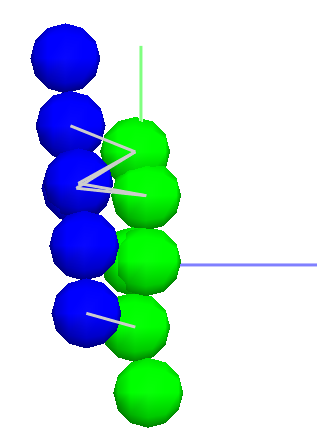
\includegraphics[scale=.15]{\fig/6Example.png}}
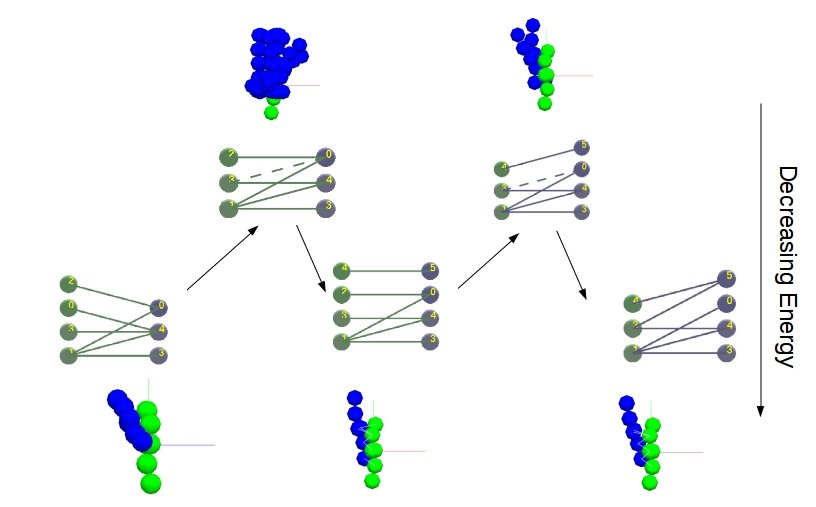
\includegraphics[scale=.4]{\fig/Paths.jpg}
\caption{A path in a toy-sized atlas. The path connects two active constraint
regions (left to right), each with 6 active constraints. The path traverses
regions with at most one less constraint. Each active constraint region is
labeled by its corresponding active constraint graph. The arrows form a path,
losing or gaining a new active constraint, from the source to the destination
active constraint regions.  The sweep view of feasible configurations of a
sample flip is shown next to each active constraint region. The left inset figure 
(\exref{\toyhelix}) shows the input molecules used for this experiment.}
\label{paths}
\end{figure}

\begin{table}[h]
\begin{tabular}{ccC{3cm}C{3cm}}\hline
$n$ & $r$ & Average length of shortest path &Average time (see text) to find shortest path\\\hline
6& 176 & 7 & 1.9 ms \\\hline
6& 145 & 6 & 2.2 ms \\\hline
20& 787 & 18 & 119ms\\\hline
\end{tabular}
\\\subcaption{\\The time on a standard laptop (see text), to find the shortest path
between two active constraint regions with 6 active constraints through $m$ 
other active constraint regions with 5 or 6 active constraints.}

\bigskip

\begin{tabular}{cccC{4cm}}\hline
$n$ & $r$ & $t$ & Average time (see text) to find number of paths\\\hline
\multirow{3}{*}{6}
				&176 & 2 & 2.02 s\\
				&176 & 4 & 4 s\\
				&176 & 8 & 6.04 s\\
				&176 & 10 & 8.08 s\\\hline
\multirow{3}{*}{20}
				& 787 & 2 & 6 min\\
				& 787 & 4 & 11.58 min\\
				& 787 & 8 & 18.04 min\\
				& 787 & 10 & 27.44 min\\\hline
\end{tabular}
\\\subcaption{\\The time on a standard laptop (see text), to find the number of
paths of length $t$, between all pairs of active constraint regions with
6 active constraints, in a toy atlas with $r$ active constraint regions with 6
active constraints.}
\caption{Finding paths between active constraint regions}
\label{table:paths}
\end{table}


This experiment was performed on two example point-sets with $n=6$ (\exref{\toyhelix})
and $n=20$ (\exref{\bighelix}). In the first experiment, the shortest
path between 100 randomly chosen pairs of active constraint regions with 6
active constraints are found. As shown in Table \ref {table:paths}, for the $n = 6$
example input, it took an average of 2 ms to find the shortest path, and the
average length of the shortest path was 6. For the $n=20$ example input, it
took an average of 119 ms to find the shortest path with the average length of
the shortest path being 18. These results can be reproduced using the test
driver (see Section 2.4 of the user guide)

In the second experiment, the number of paths of length $t$ in a toy
atlas between all pairs of active constraint regions are found. This toy atlas had $r$
active constraint regions with 6 active constraints. As shown in Table \ref
{table:paths}, for the example input with $n=6$, the number of paths
of length 10 were found in 8 seconds and the number of paths for the $n=20$ input in 27
minutes. These results can be reproduced using the test driver (see Section 2.4
of the user guide)
 

\subsection{Coverage and Sample Size Compared to MC}
In this section we sketch results from \cite{Ozkan2014MC} comparing EASAL and
its variants to the Metropolis Markov chain Monte Carlo (MC) algorithm for
sampling a portion of the landscape of two point-sets arising from protein
motifs (transmembrane helices, \exref{\bighelix}).  In that paper, the
effectiveness of EASAL in sampling crucial but narrow, low effective
dimensional regions is demonstrated by showing that EASAL provides similar
coverage as the traditional methods such as MC but with far fewer samples. For
determining coverage, it is sufficient to sample only the interior of an active
constraint region having 1 active constraint, without generating its children. 


EASAL variants EASAL-1, EASAL-2, EASAL-3, and EASAL-Jacobian differ in their
sampling distributions in the Cayley space and by extension in the Cartesian
space.  EASAL-1 samples the Cayley space uniformly. Since energy is directly
related to distance, this does uniform sampling across energy levels.  This
however, skews the sampling in the Cartesian space. EASAL-2 uses a step size
inversely proportional to the Cayley parameter value. This samples more densely
in the interiors of the active constraint region and near tetrahedral bounds.
This is useful if we want to sample densely at places where degeneracies such
as flip intersections (so called conformational shifts and tunneling) are
likely to occur.  EASAL-3 uses a step size linearly proportional to the Cayley
parameter value.  This samples densely close to the boundaries. This is useful
if we want to sample densely at lower energy values.  EASAL-Jacobian uses a
sophisticated adaptive Cayley sampling method to force uniform sampling in the
Cartesian space. This is essential to compute volumes and thereby entropy and
free energy accurately. A comparison of how sampling in the Cayley space
relates to sampling in the Cartesian space, for these variants of EASAL, is
shown in \figref{fig:nonuniform}.




\begin{table}[h]
\resizebox{\columnwidth}{!}{%
\begin{tabular}{lcccccc}\hline
	sampling method & EASAL-1 &EASAL-2& EASAL-3& EASAL-Jacobian& MC &MultiGrid\\\hline
$\varepsilon$-coverage& $\lceil 0.97\rceil$ & $\lceil 1.14\rceil$& $\lceil 1.20\rceil$& $\lceil 0.66\rceil$ &$\lceil0.31\rceil$&N/A\\\hline
	Coverage percentage &92.06\% &92.42\% &74.08\% &99.53\% &99.96\%&N/A\\\hline
	Number of Samples & 100k & 40k & 30k & 1 million & 100 million&12 million\\\hline
	Ratio percentage & 3.56\%& 5.17\%& 2.97\% &3.45\% &1.29\%&N/A\\\hline
\end{tabular}
}
\caption{Comparison of EASAL variants with MC with respect to coverage and number
of samples for the two transmembrane helices shown in
\figref{fig:3Input} \protect\citeA{Ozkan2014MC}. 
Here, $\varepsilon$ is computed as described in the text.}
\label{table:coverage}
\end{table}


\begin{figure}[h]
\centering
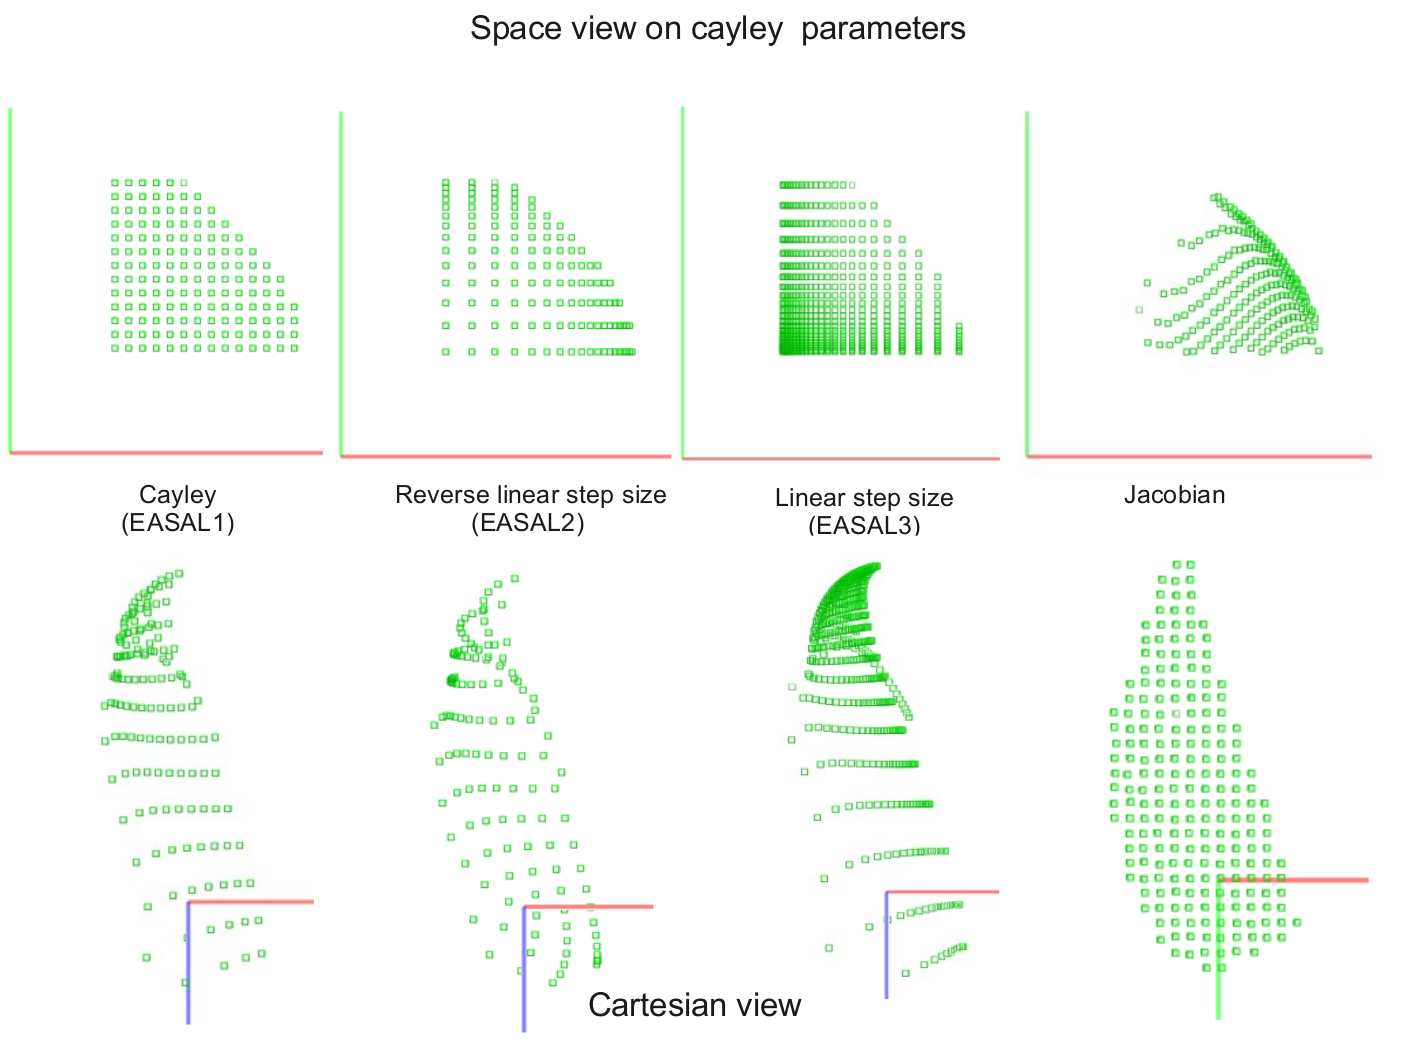
\includegraphics[scale=0.2]{\fig/NonUniformCayley.png}
\caption{Comparison of sampling in Cayley v/s Cartesian space in variants of
EASAL for a 2D active constraint region in the atlas for the example in
\figref{fig:3Input} \protect\citeA{Ozkan2014MC}. The axes in the top
	figure are the two Cayley parameters. In the bottom figure, 
	the projection is on the $xy$ coordinates of the
centroid of the second point-set with the centroid of the first point-set fixed
at the origin.}
\label{fig:nonuniform}
\end{figure}


\begin{figure}
\centering   %%% not \center
\subfigure[MC]{\label{fig:a}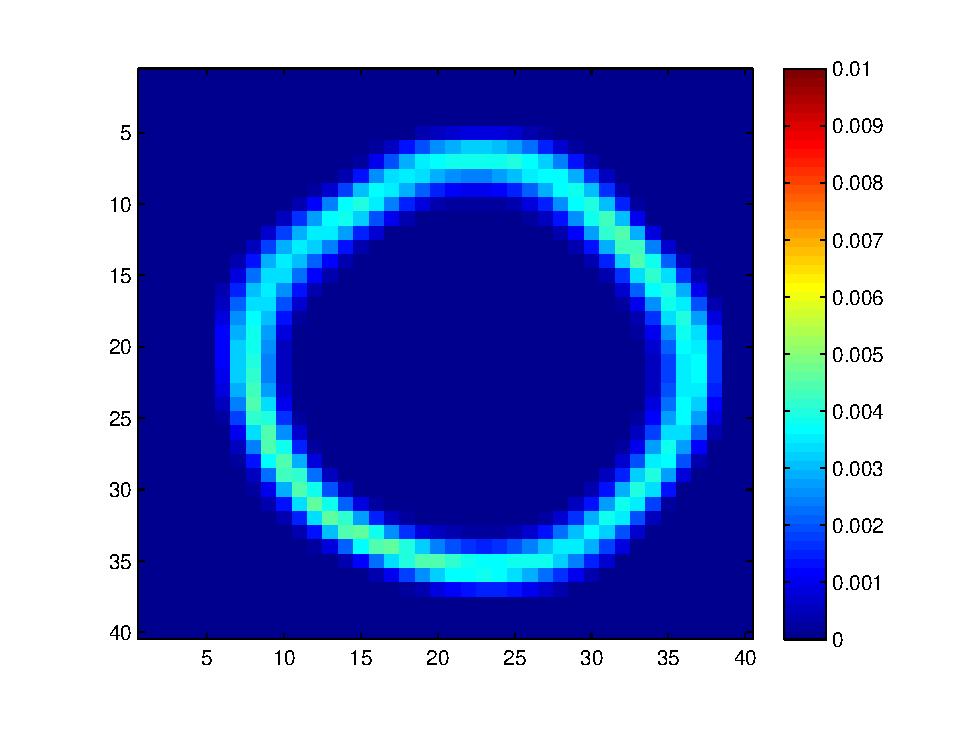
\includegraphics[scale=0.25]{\fig/MC.eps}}
\subfigure[MultiGrid]{\label{fig:b}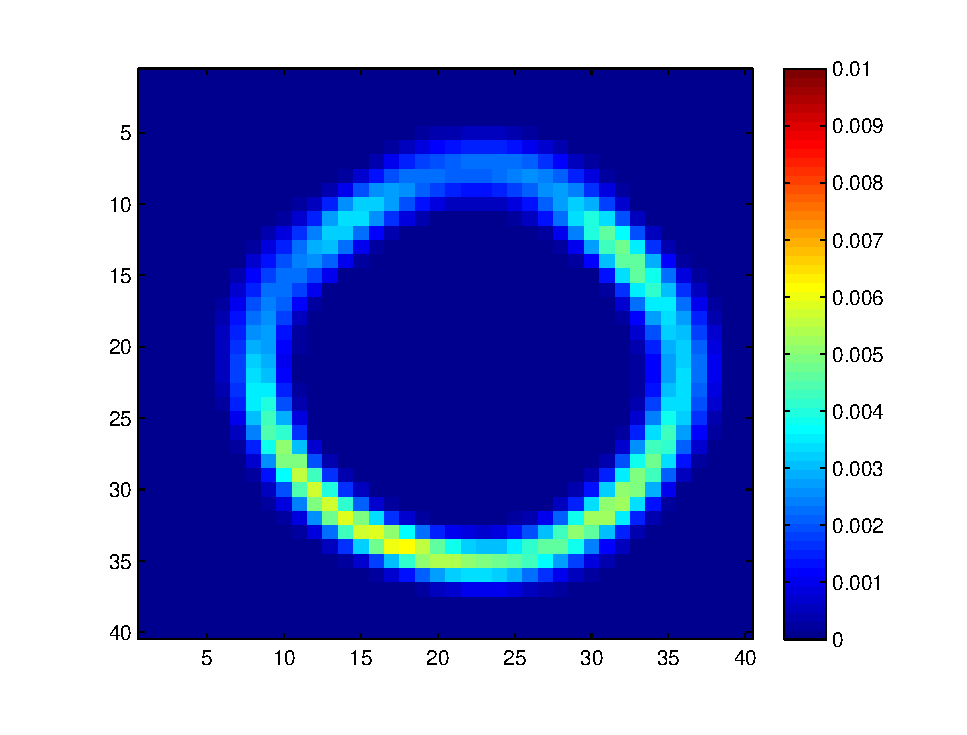
\includegraphics[scale=0.25]{\fig/MultiGrid.eps}}
\subfigure[EASAL-1]{\label{fig:c}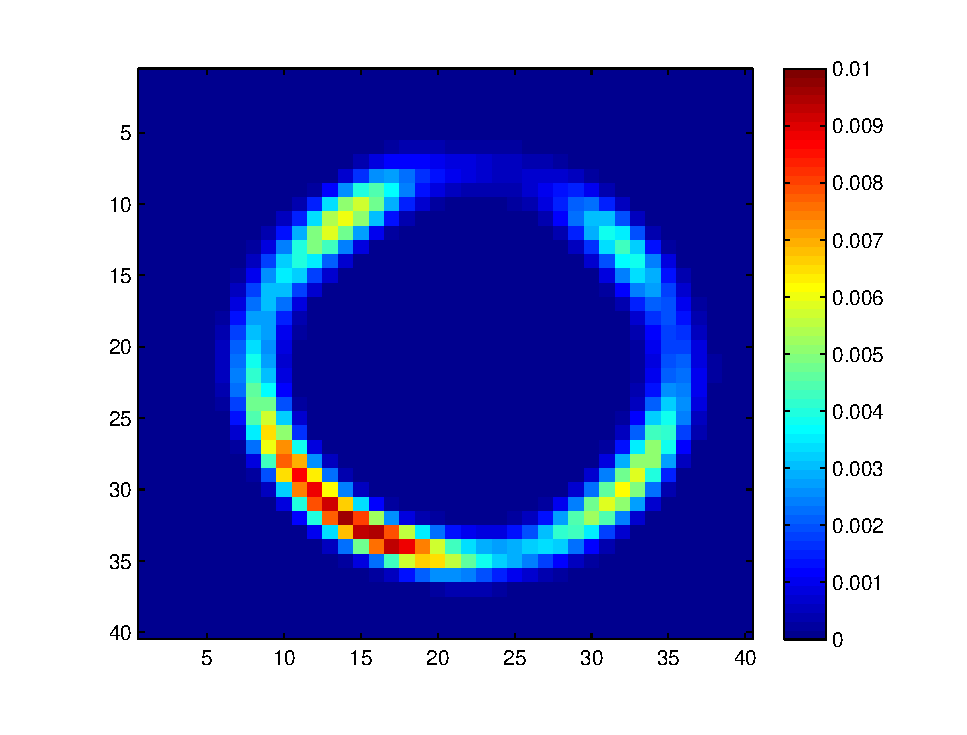
\includegraphics[scale=0.25]{\fig/EASAL1.eps}}
\subfigure[EASAL-2]{\label{fig:d}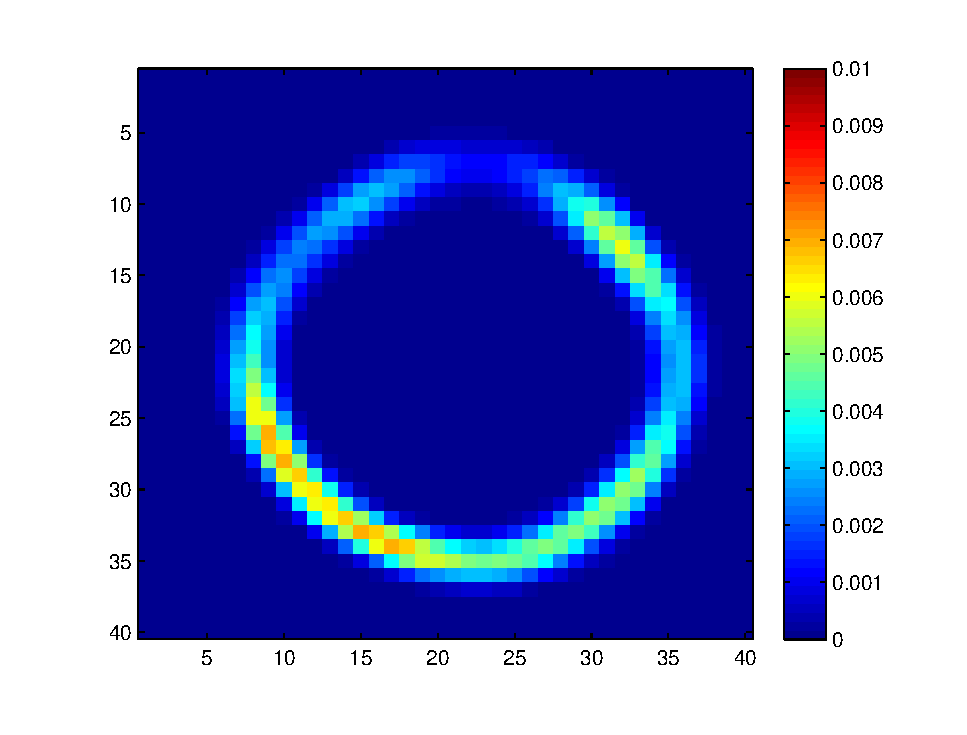
\includegraphics[scale=0.25]{\fig/EASAL2.eps}}
\subfigure[EASAL-3]{\label{fig:e}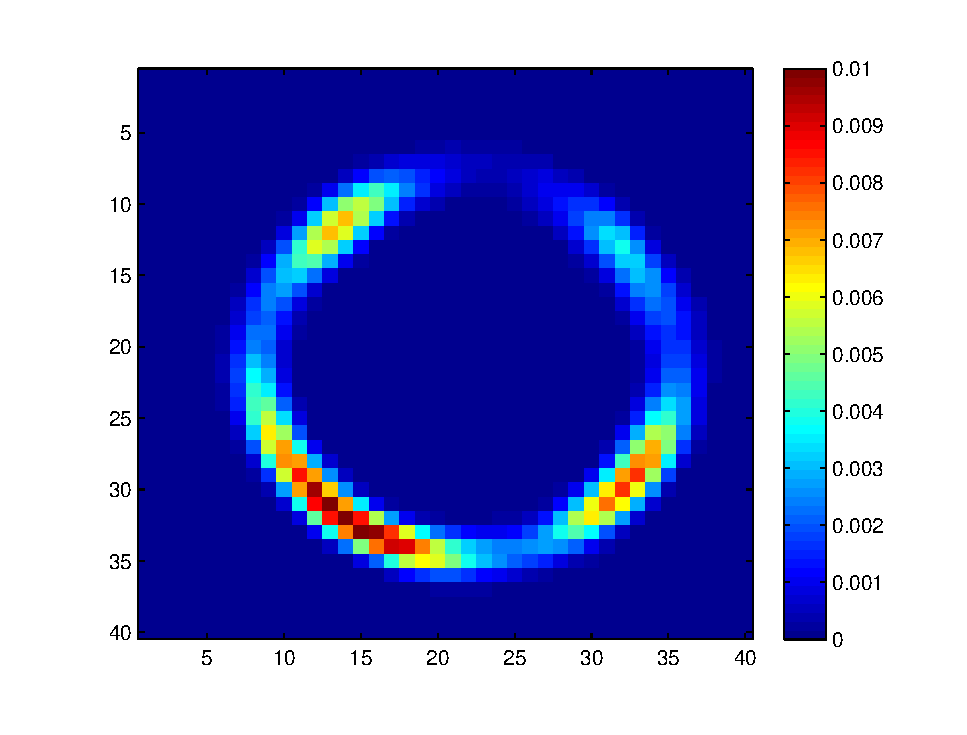
\includegraphics[scale=0.25]{\fig/EASAL3.eps}}
\subfigure[EASAL-Jacobian]{\label{fig:f}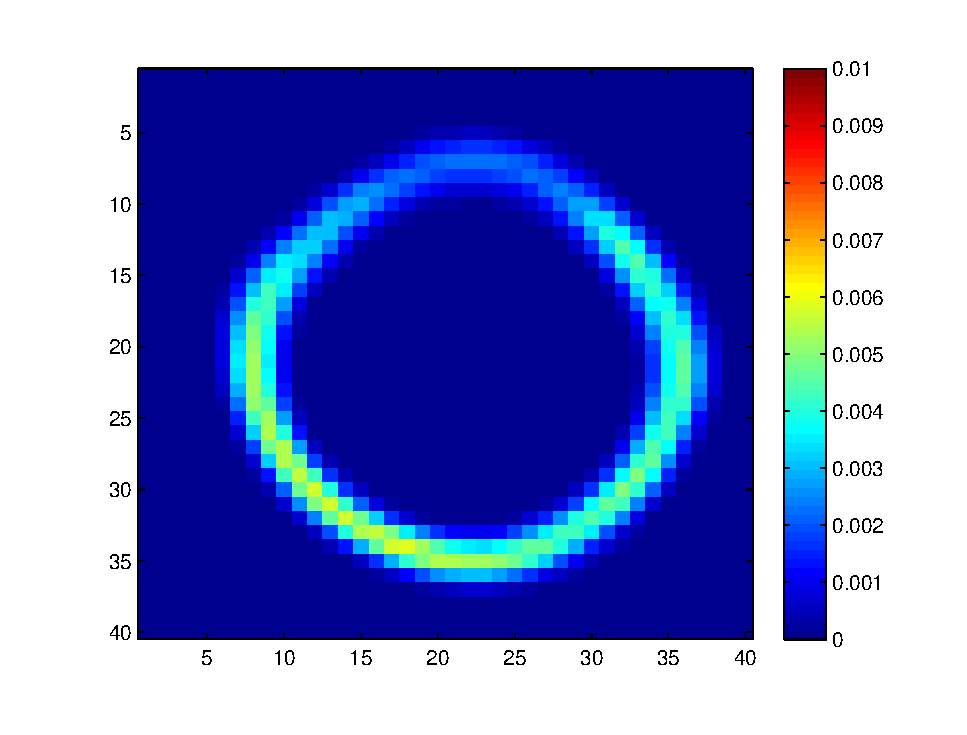
\includegraphics[scale=0.25]{\fig/EASALJacobian.eps}}
\caption{Projection in $\mathbb{R}^2$ of a configuration space for the example point-set shown
	in \figref{fig:3Input} as sampled by various methods. The
	projection is on the $xy$ coordinates of the centroid of the second
	point-set with the centroid of the first point-set fixed at the origin.
	The color scale on the right of each figure corresponds to the number
	of sampled points in a $\varepsilon$-sized cube centered around the grid
	point $(x, y)$. $\varepsilon$ is computed as described in the text \protect\citeA{Ozkan2014MC}.}
\label{fig:projectionview}
\end{figure}




The experiments were run on an Intel i5-2540 machine and the variants of
EASAL were run on a Intel Core 2 Quad Q9450 @ 2.66 GHz. and a memory of 3.9 GB.
With this setup, EASAL-1 took 3 hours 8 minutes. EASAL-2 took 4 hours 24
minutes, EASAL-3 took 10 hours 20 minutes, and EASAL-Jacobian took 14 hours 22
minutes. The methods were compared based on a their sampling coverage of a
grid. The grid was set up to be uniform in the Cartesian configuration space
and its bounds along the $X$ and $Y$ axes were -20 to 20 Angstroms, and along
the $Z$ axes were -3.5 to 3.5 Angstroms.

The input in the experiment was as follows:

\begin{enumerate}
\item[(i)] The two point-sets in the form of two rigid helices. Note that this
is the special case of Problem (\cone, \ctwo) where the points are sphere centers.

\item[(ii)] The lower bound of the pairwise distance constraint, for
all sphere pairs $i, j$ belonging to different point-sets, $dist_{ij} > 0.8 \times (\rho_i
+\rho_j)$ where $i$ and $j$ are residues, $dist_{ij}$ is the distance between
residues $i$ and $j$, $\rho_i$ and $\rho_j$ are the radii of residue spheres $i$ and
$j$ respectively.

\item[(iii)] An optional global constraint 
is the inter helical angle between the principal axes of
the two input helices, $\theta < 30^{\circ}$. Here, $\theta = a~cos(uv)$
where $u$ and $v$ are the principal axis of each point-set, i.e., $u$ and $v$
are the dominant directions in which the mass is distributed, alternatively the
eigenvectors of the inertia matrix. 

\end{enumerate}


Over 43.5 million grid configurations were generated to ensure at least one pair
was an active constraint, i.e., $dist_{ij} < \rho_1 + \rho_2 + 0.9$. Out of these, around
86\% were discarded, leaving us with about 5.8 million `good' samples.

The methods were compared based on the following parameters.
\begin{itemize}
\item [-] The epsilon coverage: a measure of how many sample points are within
an $ \varepsilon$-sphere of each grid point. Since the ambient space has
dimension 6, $\varepsilon$ is set to
$(\text{number of grid points} / \text{number of sampling points})^{1/6} /2$.

\item [-] The coverage percentage, which is the percentage of the grid
$\varepsilon$-covered by the sampling algorithm. 

\item [-] The number of samples required to achieve the given
$\varepsilon$-coverage.

\item [-] The ratio percentage: Let $s_1$ be the number of samples in a specific but randomly chosen
3 dimensional region and $s_2$ be the number of samples in all 
ancestor regions with 1 active constraint that lead to the 3 dimensional region.  The
ratio percentage is $\frac{s_1}{s_2}\times 100$.

\end{itemize}

The best method should have the highest epsilon coverage and coverage
percentage with the fewest samples. As can be seen from
Table~\ref{table:coverage}, MC gives the best coverage but requires 100
million samples. By contrast EASAL-Jacobian gives about the same relative
coverage with one million samples (1\% of MC). EASAL-2 gives a very good
coverage of 92.42\% with only 40k samples (0.04\% of MC). EASAL-2 also has the
best ratio percentage beating even MC by a large margin.
\figref{fig:projectionview} shows a 2D projection of a configuration space as
sampled by various methods for the example point-set shown in
\figref{fig:3Input}. The projection is on the $xy$ coordinates of the
centroid of the second point-set with the centroid of the first point-set fixed
at the origin. Multigrid shows grid sampling where lower dimensional regions
are repeat sampled, which is desirable. More precisely, each grid point in a
$d$ dimensional region of the atlas with $6-d$ active constraints is weighted
by $6-d$. Notice that EASAL-Jacobian and EASAL-2 approximate Multigrid (target)
better than MC.




\subsection{Viral Capsid Interaction}

\begin{figure}
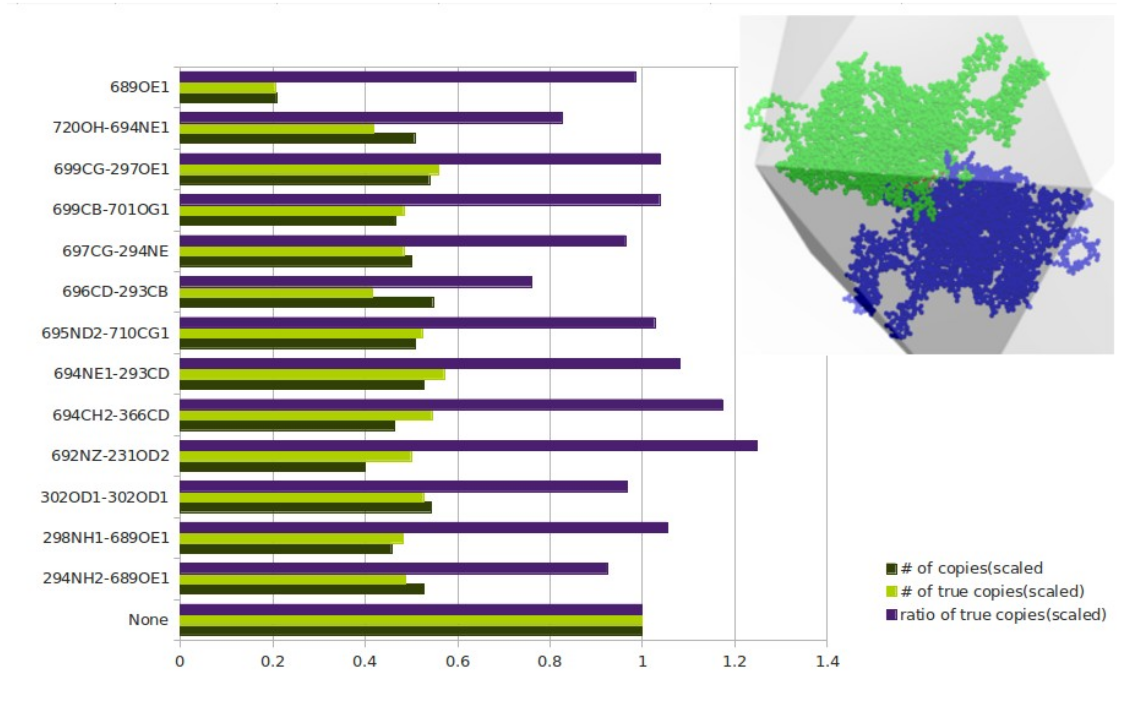
\includegraphics[scale = 0.3]{\fig/Virus1.png}

\caption{Assembly of a dimer, 2-fold interface of
the icosahedral AAV2 virus capsid. Each row corresponds to removing a
particular residue pair. These are normalized to the bottom row where no
interaction is removed and shows respectively the total number of
zero-dimensional (rigid) configurations, the number of configurations close to
the successful interface assembly configuration, and their ratio.
\protect\citeA{Wu2014Virus}.}
\label{fig:virus_comparison_dimer}
\end{figure}

\begin{figure}
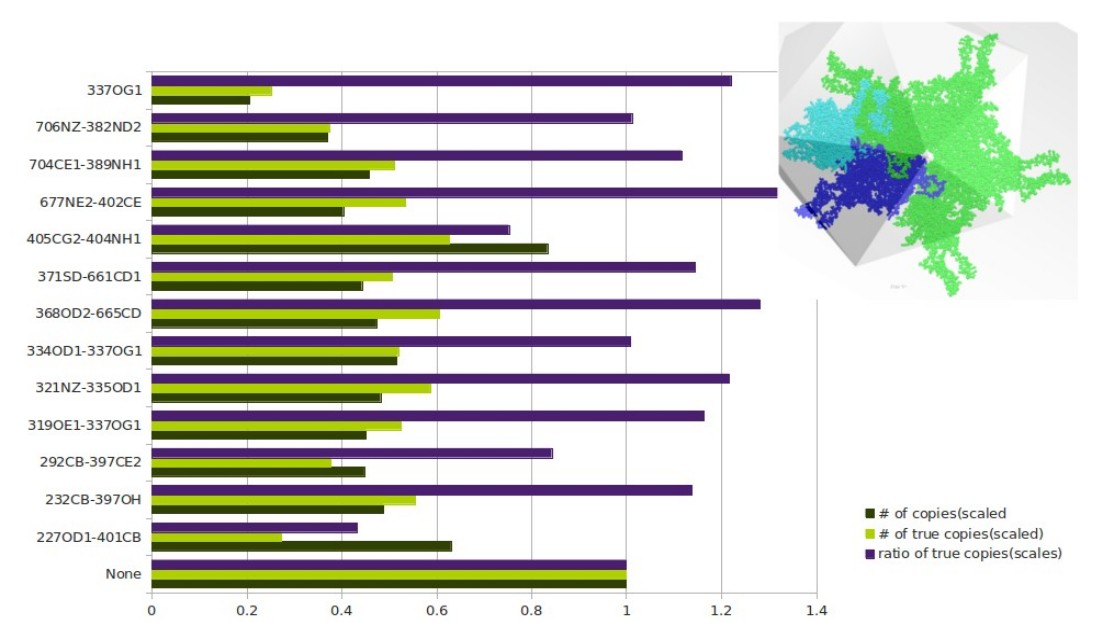
\includegraphics[scale = 0.3]{\fig/Virus2.png}
\caption{Assembly of a pentamer, 5-fold interface
of the icosahedral AAV2 virus capsid. Each row corresponds to removing a
particular residue pair. These are normalized to the bottom row when no
interaction is removed and shows respectively the total number of
zero-dimensional or rigid configurations, the number of configurations close to
the successful interface assembly configuration, and their ratio.
\protect\citeA{Wu2014Virus}.}
\label{fig:virus_comparison_pentamer}
\end{figure}



In this section we sketch results from \cite{Wu2014Virus}. EASAL has been
applied to study the configuration space of autonomous assembly into empty
shells of icosahedral T=1 viruses from nearly identical protein monomers
containing $n \ge 5000$ atoms. The robustness of such an assembly depends on
the sensitivity of free energy landscapes of inter-monomer interfaces to
changes in the governing inter-atomic interactions. The sensitivity towards
assembly disruption is generally measured by wet lab mutagenesis that disables
the chosen inter-monomer atomic interactions. \cite{Wu2014Virus} predicted this
sensitivity for the first time using EASAL to atlas the inter-monomer interface
configuration space, exploiting symmetries, and utilizing the recursive
decomposition of the large viral capsid assembly into an assembly pathway of
smaller assembly intermediates. The predictions were compared with the results
from the mutagenesis. Specifically, EASAL was used to predict the sensitivity
of 3 viral systems: Minute Virus of Mice (MVM), Adeno-Associated Virus (AAV2),
and Bromo-Mosaic Virus (BMV). For the case of AAV2, \figref
{fig:virus_comparison_dimer} and \figref {fig:virus_comparison_pentamer} show
the effect of removing a particular residue pair (the BMV results are not shown
here, \cite{unpublished}). Each row shows the total number of zero-dimensional
or rigid configurations, the number of configurations close to the successful
interface assembly configuration, and their ratio. Table \ref{table:virus}
shows comparison of the cruciality or sensitivity ranking thereby obtained to
the mutagenesis result. The highest ranked interactions output by EASAL were
validated by mutagenesis resulting in assembly disruption. The sensitivity
ranking of the dimer interface shows that all the residues marked crucial by
EASAL were confirmed as crucial by wet lab mutagenesis. The entries not listed
in the table, corresponding to non-crucial interactions, were either confirmed
as not crucial or there were no experiments performed for them. The sensitivity
ranking for the pentamer shows similar results, however experiments for some of
the residues marked by a question mark were not performed.

\begin{table}[h]

\begin{minipage}{0.45\linewidth}
\begin{tabular}{ccc}\hline
Residue1 & Residue2 & Confirmed\\\hline\hline
P293 & W694, P696 & Yes$^{*, \dag}$\\
R294 & E689, E697 & Yes $^{*, \dag, **}$\\
E689 & R298 & Yes $^{*, \dag}$\\
W694 & P293, Y397 & Yes $^{*, \dag}$\\
P696 & P293 & Yes $^{*, \dag}$\\
Y720 & W694 & Yes $^{*, \dag}$\\\hline
\end{tabular}
\subcaption{Sensitivity ranking: Dimer Interface\\}
\end{minipage}
\begin{minipage}{0.45\linewidth}
\begin{tabular}{ccc}\hline
Residue1 & Residue2 & Confirmed\\\hline\hline
N227 & Q401 & Yes $^{**}$\\
R389 & Y704 & ?\\
K706 & N382 & ?\\
M402 & Q677 & Yes $^{*, \dag}$\\
K706 & N382 & ?\\
N334 & T337,Q319 & ?\\
S292 & F397 & Yes $^{**}$\\\hline
\end{tabular}
\subcaption{Sensitivity ranking: Pentamer Interface\\}
\end{minipage}
\caption{Sensitivity ranking for the dimer and pentamer interface of AAV2. For
some residue pairs, marked by `?', there were no experiments performed and their 
cruciality is unconfirmed. $^*$ - \protect\citeA{Rayaprolu15122013}, $^\dag$ - 
\protect\citeA{mutagenesis}, $^{**}$ - \protect\citeA{Wu:00} }
\label{table:virus}
\end{table}




